\chapter{Geochemical Fingerprints of Earthquakes in Alpine Groundwater}
\label{ch:seismicity}

% ------------ 1st page ------------- %

\chaptermark{Chapter 4} % to change the headers
%\setcounter{figure}{0}
%\setcounter{table}{0}

Sébastien Giroud$^{1,2}$, Matthias S. Brennwald$^{1,3}$, Oliver S. Schilling$^{1,4}$, \\
and Rolf Kipfer$^{1,2,5}$ \\

%This chapter has been published in \textit{}.\\
%DOI: \url{}

\blfootnote{\begin{flushleft}
$^{1}$Department of Water Resources and Drinking Water, Eawag, Dübendorf, Switzerland\\
$^{2}$Institute of Biogeochemistry and Pollutant Dynamics, ETH Zürich, Zurich, Switzerland\\
$^{3}$Tracer Lab, Eawag, Dübendorf, Switzerland\\
$^{4}$Hydrogeology, Department of Environmental Sciences, University of Basel, Basel, Switzerland\\
$^{5}$Institute of Geochemistry and Petrology, ETH Zürich, Zurich, Switzerland\\
\end{flushleft}}

\vspace*{\fill}
\null{
\textcolor{gray}{
\footnotesize % Adjust size as needed
\noindent
\textbf{Acknowledgements}\\ 
We would like to express our gratitude to Gabriele Bianchetti, Alpgeo, and Cesla for their kind permission to access the wells facilities.
We thank the entire team of the Tracer Hydrogeology and Environmental Isotopes groups at Eawag for their invaluable assistance and insightful discussions.
PhD support for SG and open access funding provided by Eawag – Swiss Federal Institute of Aquatic Science and Technology.
%OSS gratefully acknowledges the funding received through SNSF-JSPS SJSSTP grant 214048.
%We sincerely thank the two reviewers for their constructive feedback, which helped improve the manuscript, and the editor for handling our submission.
}}

% ------------ 2nd page ------------- %
\newpage

\noindent
\textbf{Abstract:} Tectonic stress is known to deform the crust and perturb fluid pathways; however, its influence on deep groundwater quality remains poorly understood.
Here we present long-term, high-frequency observations of dissolved gas concentrations in an alpine geothermal field to explore how seismic activity shapes subsurface geochemical dynamics.
Our results indicate that geochemical responses become more prevalent during periods of increased seismicity, with transient shifts in groundwater composition reflected in changes to trace gas ratios such as \ce{CO2}/Ar and \ce{CH4}/Ar.
These anomalies, which occur in the absence of local ground shaking, suggest that stress-induced modulation of water mixing between chemically distinct reservoirs is occurring.
These findings offer direct evidence that seismicity alters groundwater quality through changes in flow and mixing regimes.
They underscore the value of geochemical monitoring in revealing the dynamic coupling between crustal stress and fluid systems in tectonically active environments.

\section{Introduction}
Earthquakes are among the most destructive natural disasters, causing an average of more than $6$~billion dollars in building damage annually in the USA alone and resulting in approximately \num{100000} deaths worldwide each year \citep{bilham2004urban, fema2017hazus}.
Beyond their immediate destructive impact, earthquakes can also trigger widespread environmental changes, including shifts in groundwater systems.
Observations over the past several decades have documented abrupt changes in water table levels and discharge rates in response to seismic activity \citep{shi2013coseismic, montgomery2003streamflow, king2002earthquake}.
These hydrological disturbances suggest that seismicity influences the subsurface environment well beyond the rupture zone, yet its impact on groundwater quality remains poorly understood.

In addition to hydrological shifts, geochemical changes in groundwater have been linked to seismic activity.
Anomalous concentrations of dissolved gases such as Rn, He, \ce{H2}, and \ce{CO2} have been observed before and after earthquakes \citep{segovia1989radon, igarashi1995radon, toutain1999seismo}.
Increased emissions of \ce{CO2} along fault zones have been reported following major earthquakes in regions such as along the Apennine chain in Italy, pointing to a connection between high seismicity and geochemical fluxes \citep{chiodini2020co2}.
However, many of these observations are based on sporadic sampling, making it difficult to establish whether these geochemical variations reflect a systematic response to seismicity or are site-specific anomalies \citep{toutain1999seismo}.

During periods of increased tectonic activity, significant but reversible changes in pore structure and pore pressure occur in the subsurface due to the accumulation and relaxation of elastic stress \citep{nakagomi2021stress, liu2024opposite}.
These structural changes in pore geometry are well documented in both pre- and post-seismic periods of large earthquakes, where shifts in subsurface dynamics have been shown to alter groundwater geochemistry and water levels \citep{won2019response, rutter2016aquifer}.
A notable example is the accumulation of radon in groundwater during periods of increased stress, where subsurface strain expels radon into circulating water, temporarily increasing its concentration.
This phenomenon has been observed in several seismically active regions and is attributed to stress-induced changes in pore pressure and fracture networks \citep{tarakci2014investigation, dincecco2021co2, igarashi1995radon}.
Laboratory experiments further support these findings, demonstrating that pressurized rock releases gases such as helium and argon even before mechanical failure, highlighting a potential link between subsurface stress and fluid geochemistry \citep{honda1982release, bauer2016release, bauer2019release, roques2020helium}.
These findings suggest that seismic activity could play a fundamental role in modulating groundwater composition, but direct long-term observations in deep groundwater systems remain scarce.

Recent advances in terrestrial noble gas geochemistry now allow quasi-continuous measurements of dissolved gas concentrations, including He, Ar, Kr, \ce{N2}, \ce{O2}, \ce{H2}, \ce{CH4}, and \ce{CO2}, in groundwater systems \citep{brennwald2016portable, giroud2023new}.
Here, we apply these advancements to investigate how seismic activity influences the dissolved gas composition of groundwater in a geothermal field.
We conducted continuous, high-frequency measurements of dissolved gases in thermal waters from a seismically active region in the Swiss Alps.
Using a portable mass spectrometer, we monitored \ce{H2}, \ce{He}, \ce{Ar}, \ce{Kr}, \ce{N2}, \ce{O2}, \ce{CO2}, and \ce{CH4} in deep groundwater over more than three years.
This dataset---comprising over \num{250000} measurements---provides an unprecedented experimental basis for assessing how tectonic stress and seismicity influence groundwater chemistry in fractured rock aquifers.

By analyzing the temporal evolution of dissolved gases in relation to regional seismic events, we aim to determine whether seismic activity systematically modulates groundwater geochemistry.
Specifically, we assess whether fluctuations in gas composition correlate with high seismicity and groundwater mixing dynamics.
Understanding these interactions is crucial for improving our knowledge of subsurface groundwater dynamics in seismically active regions and provides new perspectives on the broader influence of seismicity on groundwater systems and water quality.

% Results
\section{Results}
From September 2021 to January 2025, quasi-continuous dissolved gas measurements were collected from the thermal waters of wells P201 (\SI{201}{\metre} deep) and P600 (\SI{516}{\metre} deep) using a miniRUEDI instrument \citep{brennwald2016portable, giroud2023new}.
The analysis yielded a total of more than \num{250000} measurements, while the Swiss Seismological Service (SED) documented over \num{2800} seismic events within a \SI{100}{\kilo\meter} radius of Lavey-les-Bains, with moment magnitudes (M$_w$) ranging from \SIrange{-0.6}{4.2}{} \citep{sed2025earthquakes}.

Distinct changes in dissolved gas composition, particularly in the \ce{CO2}/Ar and \ce{CH4}/Ar ratios, were observed during periods of seismic activity.
The initial evidence of a systematic relationship between seismicity and groundwater composition emerged from two significant earthquakes: the Arolla (main shock on 2021-10-05 07:39, M$_w$ = 4.1) and Sanetsch (main shock on 2021-11-01 21:13, M$_w$ = 2.8) events, which occurred within \SI{50}{\kilo\meter} of Lavey-les-Bains in late 2021.

\subsection{Arolla and Sanetsch earthquakes}
In the weeks surrounding the Arolla and Sanetsch earthquakes, the dissolved gas composition in groundwater from well P201 exhibited a systematic shift (Figure~\ref{fig:arolla_sanetsch}).
Changes in the \ce{CO2}/Ar and \ce{CH4}/Ar ratios coincided with both seismic events, despite the absence of recorded seismic waves at Lavey-les-Bains.
In each case, the data form two distinct clusters, separated by a transitional phase of low data density.
This pattern suggests a shift in the geochemical equilibrium of the groundwater system linked to the seismic events.

\begin{figure}[H]
    \centering
    \includegraphics[width=0.9\textwidth]{chapters/04_chap3/figures/arolla_sanetsch.pdf}
    \caption{Dissolved gas composition in well P201 around the Arolla and Sanetsch earthquakes.
    Each panel shows \ce{CO2}/Ar versus \ce{CH4}/Ar ratios, with color indicating the time of measurement relative to the earthquake (blue = earlier, yellow = later).
    Red circles highlight periods of lower data density.
    }
    \label{fig:arolla_sanetsch}
\end{figure}

The Euclidean Distance (EuD) analysis (subsection \ref{methods:EuD} for details) revealed a pronounced increase in EuD values in the days preceding both earthquakes (Figure~\ref{fig:EuD_SanAr}).
This shift indicates a measurable change in groundwater composition associated with both seismic events, independent of direct ground shaking effects. \citep{giroud2023new}

\begin{figure}[H]
    \centering
    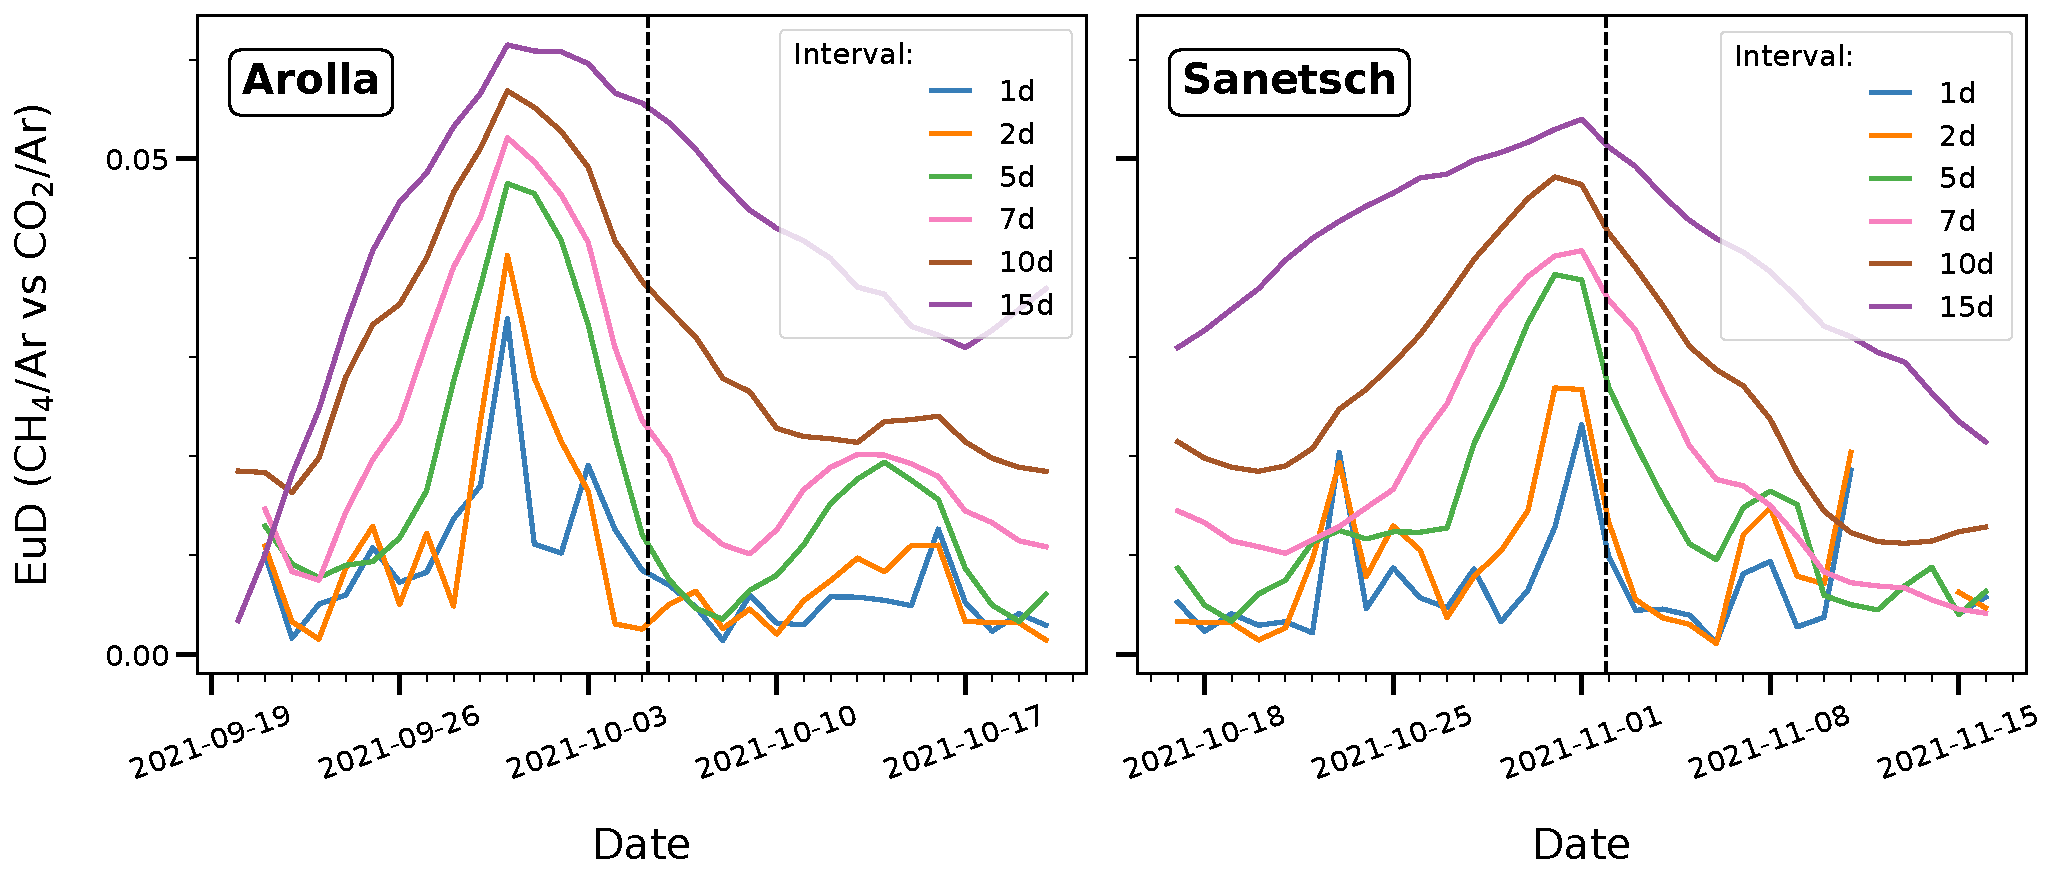
\includegraphics[width=0.9\textwidth]{chapters/04_chap3/figures/article_EuD_SanAr.pdf}
    \caption{EuD values for \ce{CO2}/Ar vs. \ce{CH4}/Ar ratios in well P201 around the Arolla and Sanetsch earthquakes (dashed vertical lines).
    EuD were computed at a \SI{1}{\day}-resolution using time intervals ranging from \SIrange{1}{15}{\day}.
    }
    \label{fig:EuD_SanAr}
\end{figure}

\subsection{Euclidean distance in P201 over time}
To assess whether the relationship between seismic activity and groundwater composition extends beyond the Arolla and Sanetsch events, we applied EuD analysis to the entire time series from September 2021 to January 2025.
EuD was calculated using a 7-day moving window at a 1-day resolution, based on \ce{CO2}/Ar and \ce{CH4}/Ar.

To compare these changes to regional seismicity, earthquakes were filtered by selecting events with M$_w \geq 2.0$ and epicentral distances within \SI{50}{\kilo\meter} of Lavey-les-Bains.
This selection mirrors the characteristics of the Arolla and Sanetsch earthquakes and follows thresholds previously used in similar studies of geochemical responses to seismicity \citep{chiodini2020co2}.

Over the full monitoring period, distinct EuD peaks are evident (Figure~\ref{fig:EuD_EuD7}).
These peaks, particularly those reaching higher amplitudes, tend to coincide with periods of increased regional seismic activity.
This recurring pattern is consistent with previous findings in other tectonically active regions, such as in Japan \citep{giroud2023new}.

Figure~\ref{fig:EuD_EuD7} also includes close-up views of the EuD signal in the immediate vicinity of each selected earthquake.
The inset shows the EuD evolution centered on individual seismic events, enabling a direct visual comparison of groundwater composition changes before and after each rupture.
In several cases, localized EuD increases and elevated short-term variability are evident around the time of the earthquake.
The average EuD across all events peaks near the seismic occurrence, indicating a general increase in EuD near earthquake timing.
The associated standard deviation also increases substantially, reflecting considerable variability in the geochemical response across different events.

\begin{figure}[H]
    \centering
    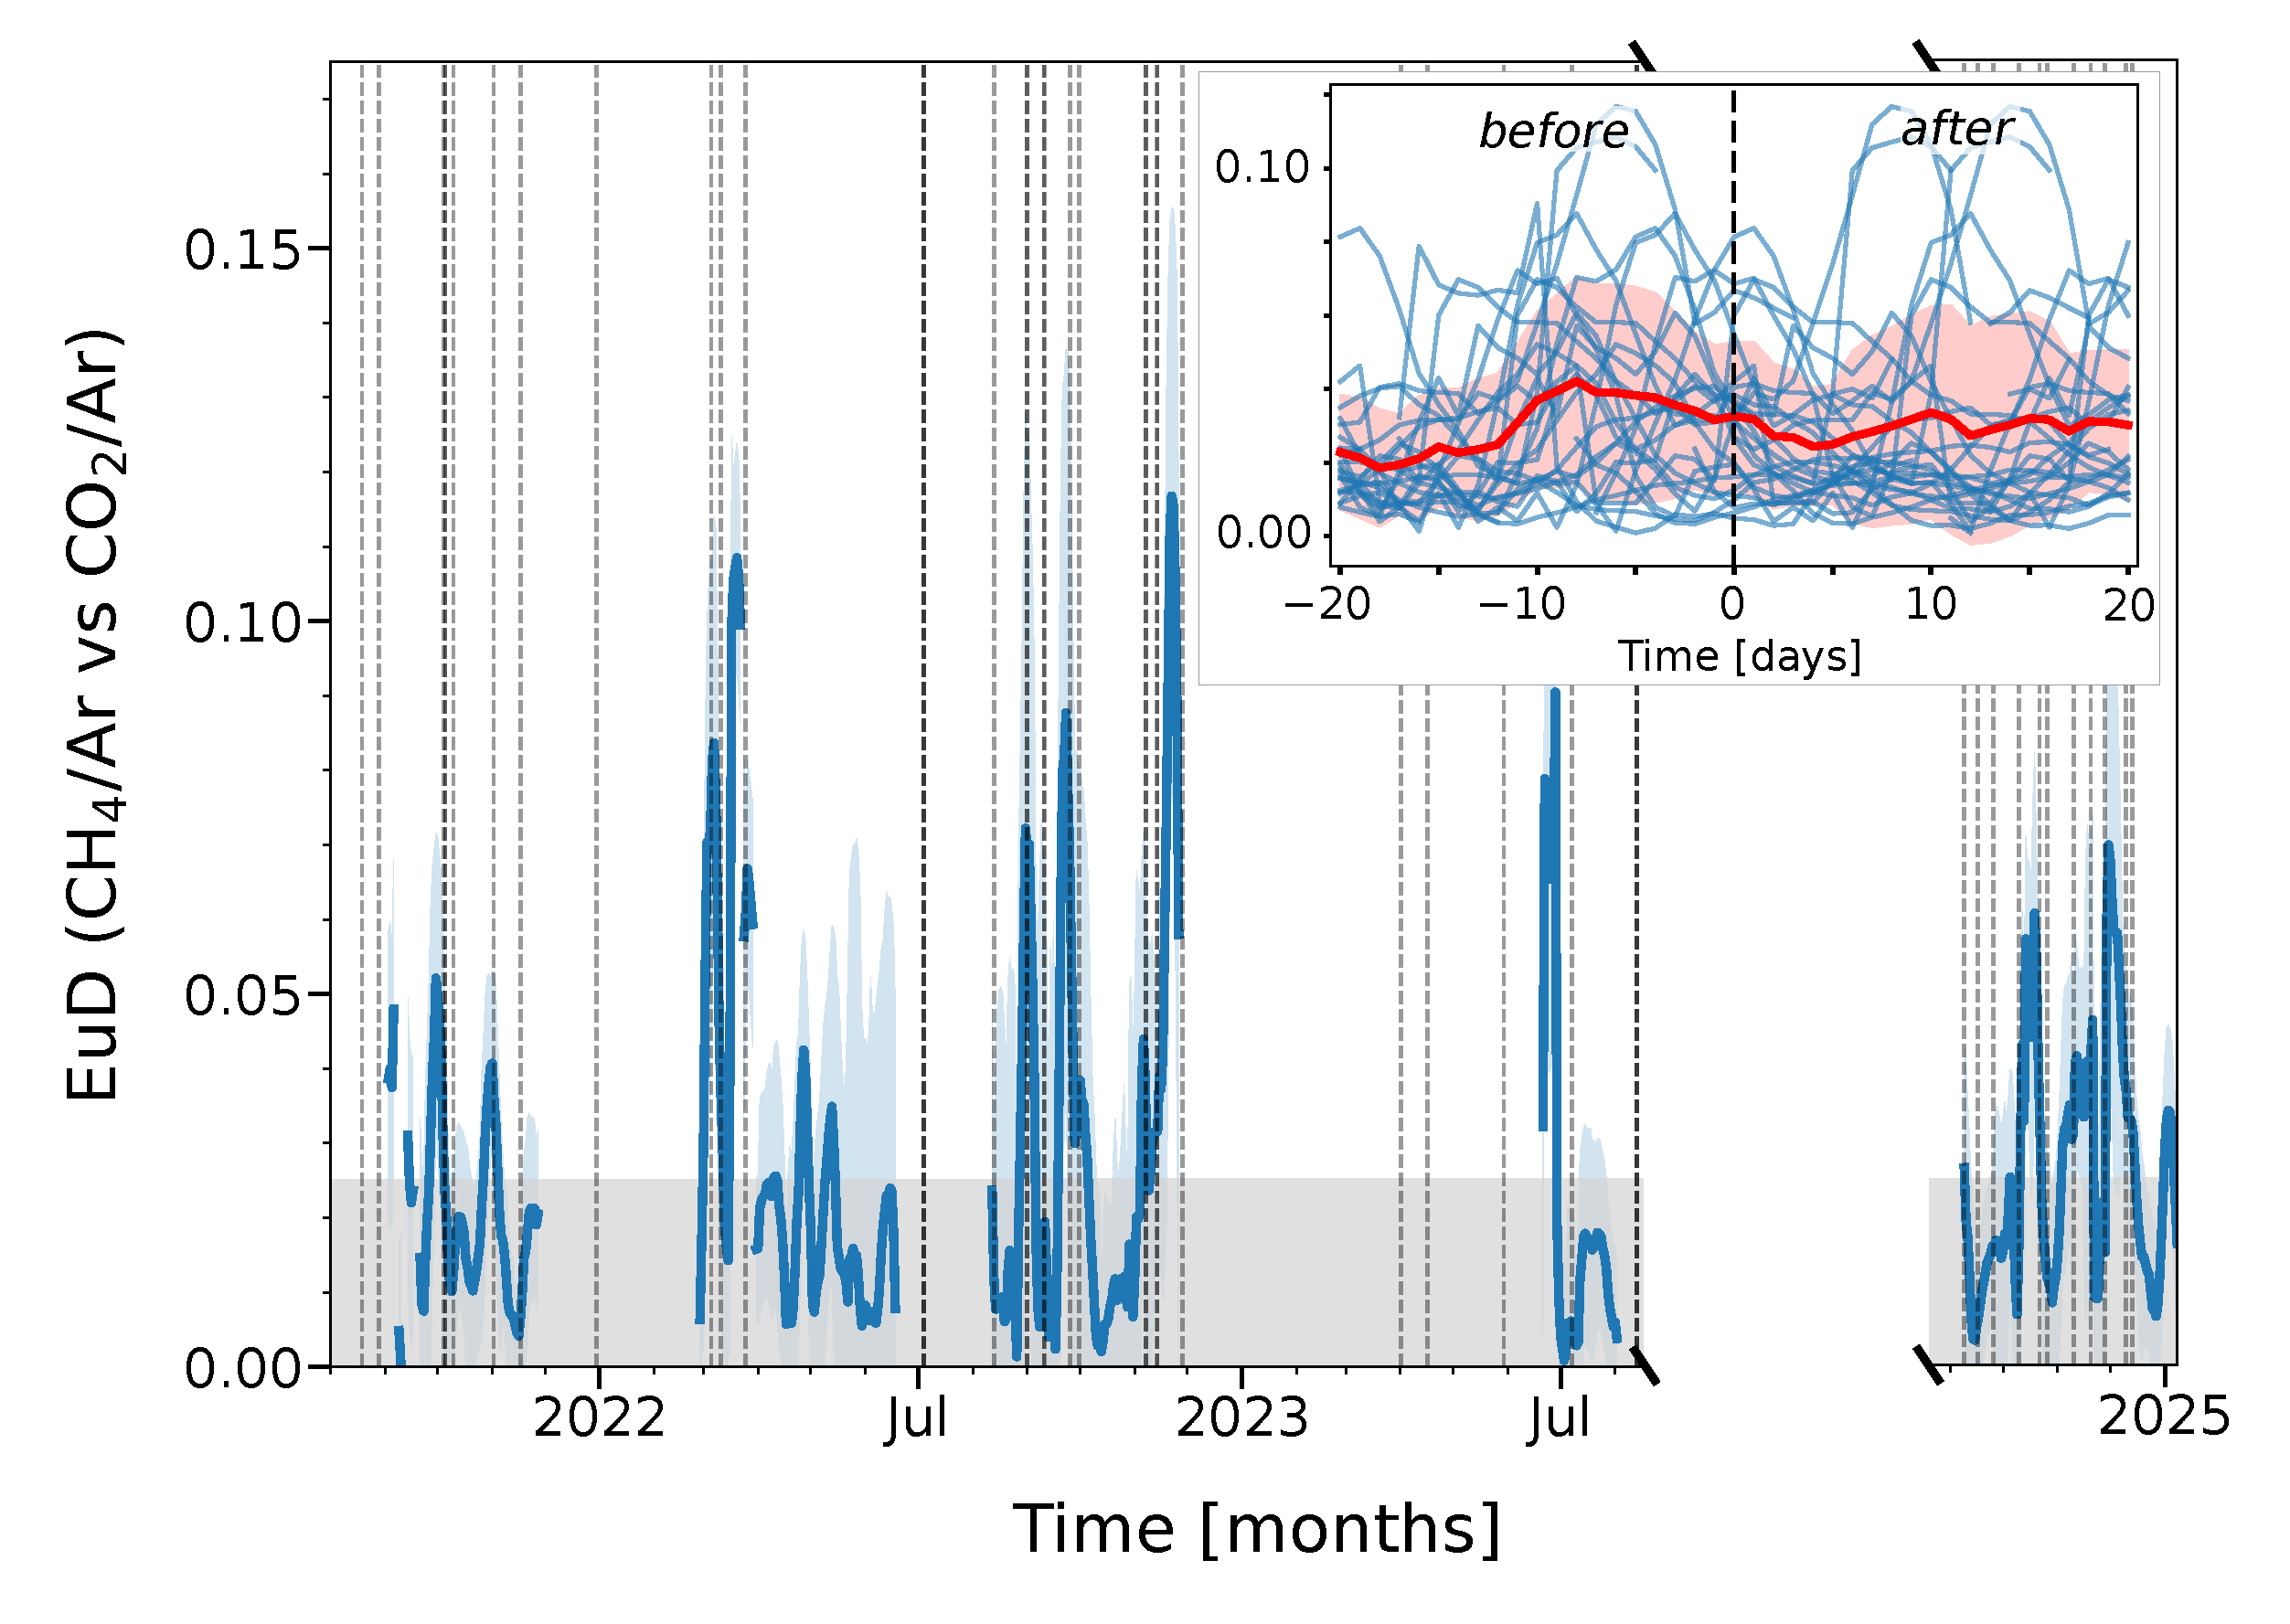
\includegraphics[width=0.8\textwidth]{chapters/04_chap3/figures/full_EuD_7_article.pdf}
    \caption{
    EuD values (blue) for \ce{CO2}/Ar vs. \ce{CH4}/Ar ratios in well P201, calculated using a 7-day interval and 1-day resolution from September 2021 to January 2025.
    The blue shaded area shows the propagated uncertainty in EuD values.
    The gray band indicates the average propagated uncertainty, used as a noise threshold.
    Earthquakes (M$_w \geq 2.0$) within \SI{50}{\kilo\meter} of Lavey-les-Bains are marked by vertical dashed lines.
    The inset displays EuD values centered on individual earthquakes, excluding events with foreshocks or aftershocks within $\pm \SI{2}{\day}$ of the main shock.
    The red line represents the average EuD across all aligned events, with the red shaded area showing the associated standard deviation.
    }
    \label{fig:EuD_EuD7}
\end{figure}

\subsection{Statistical Comparison Between Observed and Synthetic Distributions}
To evaluate whether the temporal association between seismicity and changes in groundwater composition is statistically significant, we compared the observed distribution of time differences between EuD maxima and nearby earthquakes to a synthetic distribution generated from randomly distributed events.
The analysis included earthquakes within \SI{50}{\kilo\meter} of Lavey-les-Bains and with M$_w \geq 2.0$, matching the characteristics of the Arolla and Sanetsch earthquakes.

The observed distribution (Figure~\ref{fig:distributions_P201}) shows a marked asymmetry, with most EuD maxima occurring prior to the corresponding earthquake.
This asymmetry toward negative time lags suggests that changes in groundwater chemistry tend to precede regional seismic events.
Based on the empirical offset observed between the Arolla earthquake and its corresponding EuD maximum (6 days), we applied a maximum time lag threshold of \SI{18}{\day} to both distributions, consistent with a 3$\sigma$ window.

When comparing the observed and synthetic distributions using a two-sample Kolmogorov-Smirnov test (subsection \ref{methods:stats}), the null hypothesis---that both distributions originate from the same population---was rejected at the \SI{5}{\percent} significance level (\textit{p} = 0.0497).
This result supports the conclusion that the temporal alignment between EuD maxima and earthquakes is unlikely to be due to chance.

\begin{figure}[H]
    \centering
    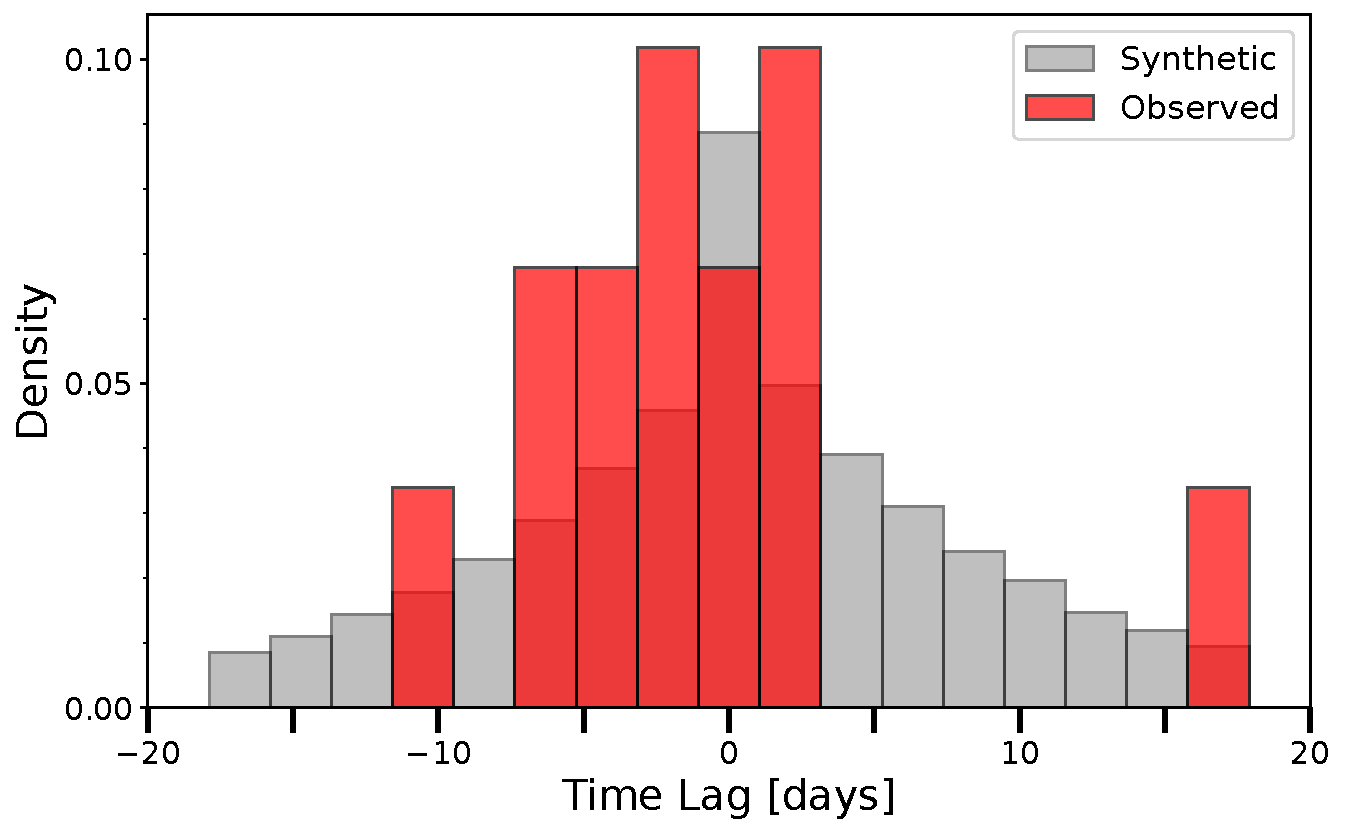
\includegraphics[width=0.75\textwidth]{chapters/04_chap3/figures/distribution_earthquakes_wo_outliers_well_201.pdf}
    \caption{Distribution of time lag between EuD maxima in well P201 and regional earthquakes (red, observed data; M$_w \geq 2.0$, within \SI{50}{\kilo\meter} of Lavey-les-Bains), compared to a synthetic distribution of randomly generated earthquakes (grey, synthetic data; \num{10000} iterations).
    A maximum time lag threshold of \SI{18}{\day} was applied to both distributions.
    Negative values indicate that EuD maxima occurred before the corresponding earthquake, and positive values indicate they occurred after.
    Both distributions are centered on zero.
    }
    \label{fig:distributions_P201}
\end{figure}

\subsection{Comparison Between Shallow and Deep Groundwater Responses}
To evaluate whether groundwater response to seismicity varies with depth, we applied the same EuD analysis to dissolved gas data from well P600 (\SI{516}{\metre} depth).
The analysis used identical parameters and selection criteria as for P201, including earthquake magnitudes (M$_w \geq 2.0$), epicentral distance (\SI{50}{\kilo\meter}), and a maximum time lag of \SI{18}{\day} between seismic events and EuD maxima.

In contrast to P201, no systematic relationship was observed in P600.
EuD maxima did not consistently align with seismic events, and the distribution of time differences was statistically indistinguishable from the synthetic reference model (Figure~\ref{figSI:distributions_P600}).
This pattern held throughout the full monitoring period, indicating a persistent difference in response between the two wells.

% Discussion
\section{Discussion}
Seismic activity is known to alter the subsurface by transiently modifying pore structures and fluid pathways through elastic stress accumulation and release \citep{nakagomi2021stress, liu2024opposite}.
These stress-driven changes have been linked to hydrological responses such as fluctuations in groundwater levels and geochemical anomalies in both natural systems and laboratory settings \citep{rutter2016aquifer, bauer2016release}.
In particular, the release of trace gases like He and Ar prior to mechanical failure suggests that geochemical signals may reflect early changes in subsurface conditions before rupture \citep{roques2020helium}.

Our data from Lavey-les-Bains extend these insights to deep alpine groundwater systems.
In well P201, repeated shifts in dissolved gas compo-sition---quantified by changes in \ce{CO2}/Ar and \ce{CH4}/Ar ratios---align with increased regional seismicity.
These signals occur without detectable ground shaking, indicating sensitivity to stress accumulation rather than coseismic rupture.
The spatial and temporal alignment of these anomalies with nearby earthquakes, and their systematic absence in randomized distributions, points to a causal relationship.

We interpret these observations as the geochemical expression of stress-induced modulation of groundwater flow paths.
The Lavey-les-Bains geothermal system is characterized by the mixing of chemically distinct water sources, as shown by hydrogeological models and tracer studies \citep{sonney2009numerical, giroud2025microbio}.
A deep, geochemically evolved component interacts with younger, less mineralized groundwater between approximately \SIrange{200}{500}{\metre} depth.
If seismic stress modifies fracture connectivity or permeability at depth, even subtly, it could temporarily shift the balance between these sources.
Such mixing changes would alter the concentration of minor gases like \ce{CO2} and \ce{CH4}, whose low abundance and strong source dependency make them sensitive indicators of water origin.

This framework explains both the observed correlation in P201 and the absence of a similar signal in P600.
Unlike P201, well P600 predominantly taps the deep, evolved component with minimal contribution from the shallower, less mature water.
Its relative geochemical stability suggests a more isolated flow regime, less affected by transient shifts in mixing.
The contrast between the two wells thus supports the idea that seismic stress alters groundwater quality by modulating the mixing dynamics within a heterogeneous flow system.

These findings suggest a mechanism by which regional tectonic loading can exert a measurable influence on deep groundwater quality.
The absence of direct rupture or local shaking highlights the role of elastic strain fields as drivers of subsurface hydrodynamics.
While our interpretation is site-specific, it offers a conceptual framework that could be tested in other tectonically active hydrothermal fields.
High-frequency geochemical monitoring---particularly in settings where distinct water components interact---may reveal similar stress-induced signals, offering a new lens on crustal deformation and its hydrological consequences.

% Conclusion
\section{Conclusion}
This study demonstrates that regional seismicity can transiently alter deep groundwater quality by modulating subsurface mixing dynamics between chemically distinct water sources.
The observed geochemical fluctuations---occurring without local rupture and often preceding the seismic events---highlight elastic strain as a powerful control on crustal hydrology.
These results offer a new perspective on how tectonic stress can influence fluid pathways in geothermal fields.

A critical question emerging from this work is whether such preseismic geochemical changes represent a consistent signature of impending rupture.
Investigating this possibility across other tectonically active regions will be essential for assessing the broader relevance of these signals.
High-frequency, long-term geochemical monitoring in systems with known water mixing could thus not only deepen our understanding of crustal deformation, but also inform the development of new approaches to earthquake forecasting.

\section{Methods}
\subsection{Site}
Lavey-les-Bains (\SI{46.204359}{\degree}N, \SI{7.017797}{\degree}E) is located in the Swiss Alps, in one of the most seismically active areas of Switzerland.
The thermal field is fed by hot groundwater that rises through the fractured crystalline gneiss of the Aiguilles Rouges massif, a geological formation that straddles the French and Swiss Alps.
This geothermal field facilitates mixing between ancient, hot groundwater and cooler, less evolved waters at depths of \SIrange{200}{500}{\meter}, with reservoir temperatures estimated at \SIrange{110}{120}{\celsius}. \citep{sonney2009numerical, wanner2019quantification, giroud2025microbio}.

Two key wells, P201 (\SI{201}{\meter} depth, \SI{51}{\celsius}) and P600 (\SI{516}{\meter} depth, \SI{64}{\celsius}), supply thermal water to the local spa.
P201 taps shallower strata and exhibits greater seasonal variability due to interactions with colder surface waters, while P600 taps deeper, more stable mixing ratios \citep{sonney2009numerical, giroud2025microbio}.

\subsection{Dissolve gas quantification}
Thermal waters from wells P201 and P600 were directly connected to a membrane module (Liqui-Cel\textsuperscript{\texttrademark}, 3M\textsuperscript{\texttrademark}) with a flow rate of approximately \SI{1}{\liter\per\minute}.
A portable gas equilibrium membrane inlet mass spectrometer (miniRUEDI, \cite{brennwald2016portable}) was attached to the headspace of the membrane module to measure dissolved gases.
To prevent water condensation in the headspace, a heating box was installed and maintained at about \SI{70}{\celsius} \citep{giroud2023new}.

The miniRUEDI was configured to measure \ce{H2}, \ce{CH4}, \ce{N2}, \ce{O2}, \ce{^{40}Ar}, and \ce{CO2} with the Faraday cup detector, while \ce{^4He} and \ce{^{84}Kr} were measured with the electron multiplier detector.
The time resolution was approximately \SI{10}{\minute}.
Raw data from the mass spectrometer were calibrated to partial pressures using either atmospheric air \citep{porcelli2002overview} or a gas mixture standard (\SI{97}{\percent} \ce{N2}, \SI{1}{\percent} \ce{H2}, \SI{1}{\percent} \ce{CO2}, and \SI{1}{\percent} \ce{CH4}; \cite{tomonaga2019montterri}).


\subsection{Euclidean Distance Analysis}\label{methods:EuD}
To systematically quantify temporal variations in gas composition and distinguish short-term geochemical perturbations from long-term seasonal trends, we applied the Euclidean distance (EuD) as a metric.
This approach allows for the detection of subtle changes in dissolved gas concentrations that may be associated with seismic activity while filtering out transient or seasonal fluctuations and instrumental noise.  

For a given time interval (\(\Delta t\)), the EuD at a specific time \(t_0\) was computed by defining two adjacent, non-overlapping time intervals of equal length.
The first interval spans from \(t_0\) to \(t_0 + \Delta t\), while the second extends from \(t_0\) to \(t_0 - \Delta t\).
Within each interval, gas concentration measurements were averaged to obtain two mean values, \(M_1\) and \(M_2\), representing the mean gas composition for each period.
The EuD was then calculated as the difference between these two mean values, providing a quantitative measure of temporal divergence in gas composition.

This process was repeated for each successive day in the time series using a sliding window approach of resolution \SI{1}{\day}, ensuring a continuous EuD dataset that captures variations over time.
By applying this analysis to the normalized gas ratios \ce{CO2}/Ar and \ce{CH4}/Ar, we enhanced sensitivity to changes in fluid mixing within the geothermal field.
The selection of these gases was based on their low concentrations (approximately \SI{1}{\percent} of the total pressure) and their known sensitivity to subsurface processes.

\subsection{Statistical Testing}\label{methods:stats}
To construct the observed distribution, EuD peaks were identified using the \texttt{find\_peaks} function from the SciPy package.
Time lags were calculated as the difference between each EuD peak and the nearest earthquake, considering only events that satisfied the following criteria: a maximum epicentral distance of \SI{50}{\kilo\meter} from Lavey-les-Bains and a magnitude threshold of M$_w \geq 2.0$, consistent with the Arolla and Sanetsch events and previous work \citep{chiodini2020co2}.
Only earthquakes that occurred within the time span of available EuD measurements were considered.

To generate the synthetic distribution, the same number of earthquakes as in the observed dataset was randomly distributed within the EuD time series.
Time lags were then calculated between each EuD peak and the synthetic events, applying the same \SI{18}{\day} cutoff.
This process was repeated \num{10000} times to construct a null model of expected lag distributions under random association.

To ensure meaningful temporal associations, we limited the analysis to time lags within \SI{18}{\day}, based on a 3$\sigma$ threshold derived from the empirically observed \SI{6}{\day} delay between the Arolla earthquake and its associated EuD maximum.
Observed and synthetic distributions were compared using a two-sample Kolmogorov–Smirnov (KS) test (\texttt{ks\_2samp}, SciPy), with a significance threshold of \SI{5}{\percent} (\textit{p} < 0.05).

All processing steps and analysis routines are available in the associated Jupyter notebook.

\subsection{Data availability}
Seismic data were obtained from the Swiss seismological service (SED, \cite{sed2025earthquakes}).
Processed dissolved gas measurements from P201 and P600 can be found at \textcolor{red}{Eric data repository Eawag}
Python script are freely accessible at \url{https://github.com/seb-gi/earthquake_lavey.git}.